\section{Requirements Engineering}
\label{chap:Requirements Engineering}
Nach der Definition des \ac{IREB} bezeichnet das \ac{RE} die systematische 
und disziplinierte Vorgehensweise bei der Spezifikation und dem Management von Anforderungen. Das Ziel des \ac{RE} ist dabei, 
die Wünsche und Bedürfnisse der Stakeholder zu verstehen \cite[vgl. S.30]{IREB_Glossary}. Stakeholder sind Personen oder Organisationen, die die 
Anforderungen des Systems direkt oder indirekt beeinflussen oder die von dem System betroffen sind \cite[vgl. S.33]{IREB_Glossary}. 
Beispielsweise können Kunden oder Nutzer, aber auch der Gesetzgeber, potenzielle Stakeholder sein. Außerdem soll das Risiko minimiert werden, 
dass diese Wünsche und Bedürfnisse nicht oder nur unzureichend erfüllt werden \cite[vgl. S.30]{IREB_Glossary}.

Einen Teilbereich des \ac{RE} stellt das \ac{RM} dar. Dieser Prozess beschreibt die Verwaltung, Speicherung, 
Änderung sowie die Rückverfolgung von Anforderungen \cite[vgl. S.8]{IREB_Glossary}. Um den \ac{RM} Prozess zu unterstützen, können entsprechende
Tools verwendet werden. Bei der Siemens Mobility GmbH wird das Tool \ac{DOORS} verpflichtend eingesetzt \cite[vgl. S.18]{SMO-PE}. Näheres zu
\ac{DOORS} kann dem Kapitel \ref*{chap:DOORS} entnommen werden.

\subsection{Anforderungen}
Die IEEE definiert eine Anforderung wie folgt: 
\begin{quote}
    \glqq(1) A condition or capability needed by a user to solve a problem or achieve an objective.\\
    (2) A condition or capability that must be met
        or possessed by a system or system component to satisfy a contract, standard, specification, or other formally imposed documents.\\
    (3) A documented representation of a condition or capability as in (1) or (2).\grqq \cite[S.62]{IEEE_Glossary}
\end{quote}

Daher bilden Anforderung die Basis eines jeden Projekts, da diese definieren, welche Bedingungen ein System erfüllen muss bzw. welche Fähigkeiten 
es besitzen muss. Sie werden idealerweise unter Berücksichtigung und in Zusammenarbeit mit den Stakeholdern des Projekts ermittelt. Neben den 
Stakeholdern können unter anderem auch Normen, Gesetze oder Vorgänger eines Systems weitere Quellen für Anforderungen sein. Um von jedem 
Partizipierendem des Projekts verstanden zu werden, werden Anforderungen in der Regel in natürlicher Sprache formuliert. Da natürliche Sprache Raum für 
Interpretation bieten kann, muss darauf geachtet werden, dass die Anforderungen so klar und unmissverständlich wie möglich formuliert werden und dabei 
trotzdem vollständig bleiben. Zudem wird voraussichtlich nicht jeder Stakeholder über die fachlichen Kenntnisse verfügen um Fachsprache oder 
Konventionen zu verstehen, weshalb darauf verzichtet werden sollte \cite[vgl. S.2]{DOORS}. Um sicherzustellen, dass Anforderungen korrekt 
formuliert werden, wurden in der Norm ISO/IEC/IEEE 29148:2018(E) Eigenschaften definiert, welche Anforderungen erfüllen sollen. 
Diese Eigenschaften werden nachfolgend dargestellt und kurz beschrieben:

\begin{enumerate}[leftmargin=*,labelindent=16pt,font=\bfseries, nolistsep]
    \item[Notwendig] Die Anforderung definiert eine wesentliche Fähigkeit, Eigenschaft, Einschränkung und/oder einen Qualitätsfaktor \cite[vgl. S.12]{RE-ISO}.
    \item[Angemessen] Die Anforderung verfügt über einen angemessenen Detaillierungsgrad und erlaubt dabei bei der Implementierung größtmögliche Unabhängigkeit \cite[vgl. S.12]{RE-ISO}.
    \item[Eindeutig] Die Anforderung ist leicht zu verstehen, einfach formuliert und kann nur auf eine einzige Weise interpretiert werden \cite[vgl. S.12]{RE-ISO}.
    \item[Komplett] Die Anforderung ist hinreichend beschrieben und benötigt keine weiteren Informationen um verstanden zu werden \cite[vgl. S.12]{RE-ISO}.
    \item[Atomar] Die Anforderung beschreibt eine einzige Fähigkeit oder Bedingung \cite[vgl. S.12]{RE-ISO}.
    \item[Durchführbar] Die Anforderung kann innerhalb der Beschränkungen des Systems mit akzeptablem Risiko durchgeführt werden \cite[vgl. S.13]{RE-ISO}.
    \item[Verifizierbar] Die Umsetzung der Anforderung kann überprüft werden \cite[vgl. S.13]{RE-ISO}.
    \item[Korrekt] Die Anforderung ist eine genaue Darstellung des Bedürfnisses ihrer Quelle \cite[vgl. S.13]{RE-ISO}.
    \item[Konform] Die Anforderung wurde, wenn möglich, mithilfe einer genehmigten Standardvorlage und -stil verfasst \cite[vgl. S.13]{RE-ISO}.
\end{enumerate}

Um diese Eigenschaften zu erfüllen, ist es ratsam auf Vorlagen für das Schreiben von Anforderungen zurückzugreifen. Eine Anforderung, welche mithilfe
einer Vorlage verfasst wurde, könnte wie folgt aussehen:
\begin{quote}
    \glqq The <system> shall <function> <object> every <performance> <units>.\\
    E.g. The coffee machine shall produce a hot drink every 10 seconds. \grqq \cite[S.81]{DOORS}
\end{quote}

Nach einer Umfrage aus dem Chaos Report der Standish Group nennen mehr als die Hälfte der Befragten als Faktor für die Beeinträchtigung von Projekten
einen Grund, der direkt im Zusammenhang mit mangelndem \ac{RE} und \ac{RM} steht. Dazu gehören z.B. Gründe wie unvollständige Anforderungen, Nutzer nicht
ausreichend involviert, unrealistische Erwartungen oder geänderte Anforderungen und Spezifikationen \cite[vgl. S.5]{Chaos}. Gut durchgeführtes 
\ac{RE} und \ac{RM} ist also essenziell für den Erfolg von Projekten.

\subsection{Anwendungsregeln}
Eine spezielle Form von Anforderungen stellen die Anwendungsregeln dar. Diese Anforderungen werden an Komponenten gestellt, um einen sicheren
und zuverlässigen Einsatz von Komponenten im System zu gewährleisten. Dafür müssen sie von dem Kunden oder dem Projekt, welches die jeweiligen 
Komponenten nutzt, berücksichtigt werden \cite[vgl. S.9]{SMO-AR}. Alle Anwendungsregeln von Komponenten der \ac{SMO RI} in all ihrer Versionen
befinden sich zentral gespeichert in einem Projekt im Tool \ac{DOORS}. Von dort kann der zuständige System-Manager eines Projekts alle 
Anwendungsregeln von Komponenten importieren, die im jeweiligen Projekt genutzt werden. Als Nächstes muss er bewerten, welche 
Anwendungsregeln für das Projekt anwendbar sind und welche nicht. Die anwendbaren Anwendungsregeln müssen daraufhin mit einer Designlösung
abgeschlossen werden oder einem oder mehreren Teilsystemen zugeordnet werden. Diese Bewertung der Anwendungsregeln erfolgt ebenfalls in \ac{DOORS}
wie in der Abbildung \ref*{fig:BewerteteAR} gezeigt wird.

\begin{figure}[H]
    \centering
    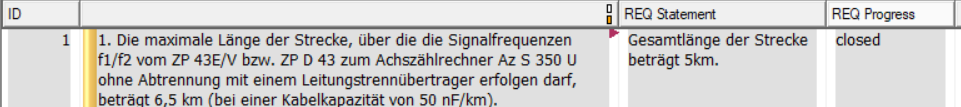
\includegraphics[width = \textwidth]{abbildungen/Bewertete AR.png}
    \caption{Bewerten einer Anwendungsregel}
    \label{fig:BewerteteAR}
\end{figure}

Dafür werden die Attribute REQ Statement und REQ Progress genutzt. Im Attribut REQ Progress kann der System-Manager eine von fünf verschiedenen
Ausprägungen wählen. Eine Auflistung und Erklärung dieser Ausprägungen kann der Tabelle \ref*{tab:REQProgress} entnommen werden. Der 
System-Manager muss daraufhin ein Statement darüber abgeben, warum er welchen REQ Progress gewählt hat. Dieses Statement wird in Textform im
Attribut REQ Statement gespeichert. Die Anwendungsregel in der Abbildung \ref*{fig:BewerteteAR} wurde beispielsweise mit closed bewertet,
da die Anwendungsregel für das Projekt anwendbar ist und zudem auch abgeschlossen ist, da die Streckenlänge, wie in der Anwendungsregel gefordert,
weniger als 6,5 km beträgt.

\begin{table}[H]
    \begin{center}
        \caption{Ausprägungen des Attributs REQ Progress \cite[vgl. S.28f.]{SMO-AR}}
        \label{tab:REQProgress}
        \begin{tabularx}{\textwidth}{|l|>{\raggedright\arraybackslash}X |}
            \hline
            \textbf{REQ Progress} & \textbf{Erklärung}\\ \hline
            not applicable & Anwendungsregel ist nicht anwendbar \\ \hline
            forwarded & Anwendungsregel soll an Subsystem weitergeleitet werden \\ \hline
            closed & Anwendungsregel auf System Design Ebene mit einem Statement abgeschlossen \\ \hline
            open &  Bewertung der Anwendungsregel noch offen \\ \hline
            compliant & Anwendungsregel anwendbar, noch nicht bewertet \\ \hline
        \end{tabularx}
    \end{center}
\end{table}